\documentclass[14px]{article}
\usepackage{xeCJK}
\usepackage[frenchb]{babel}
\usepackage[T1]{fontenc}
\usepackage[utf8]{inputenc}
\usepackage{textcomp}
\usepackage{amssymb}
\usepackage[ruled,longend]{algorithm2e}
\usepackage{amsmath}
\usepackage{latexsym}
\usepackage{fancyhdr}
\usepackage{geometry}
\usepackage{setspace}
% Image
\usepackage{graphicx}
\usepackage{subfigure}
% wrap
\usepackage{wrapfig}

\renewcommand{\baselinestretch}{1.2}

\begin{document}
	\setlength{\parindent}{0pt}
	\begin{titlepage}
		
		\begin{center}
			% Upper part of the page
			
\includegraphics[width=0.35\textwidth]{logo.png}\\[1cm]
			
			\textsc{\Large Rapport de APS}\\[0.5cm]
			
			% Title
			
			{ \huge \bfseries Analyse des Programmes et Sémantique}\\[0.4cm]
			
			% Author and supervisor
			\begin{minipage}{0.4\textwidth}
				\begin{flushleft} \large
					\emph{Author:}\\
					Qiwei \textsc{XIAN}
				\end{flushleft}
			\end{minipage}
			\begin{minipage}{0.4\textwidth}
				\begin{flushright} \large
					\emph{Professeur:} \\
					\textsc{Pascal.manoury}
				\end{flushright}
			\end{minipage}
			
			\vfill
			% Bottom of the page
			{\large \today}
		\end{center}
		
	\end{titlepage}
	\clearpage
	
	\tableofcontents
	\thispagestyle{empty}
	\clearpage
	
	\pagestyle{fancy}
	\lhead{APS0}
	\rhead{\thepage}
	\fancyfoot{}
	
\section{APS0}
\subsection{Etape1. Analyse lexicale}
Pour l'étape d'analyse lexicale, j'ai créé les associations entre les mots clefs qui peuvent être utilisé dans APS0 avec les \textbf{tokens} qui sont définits dans \textbf{parser.y}.

Après cet étape, l'interprèteur de APS0 reconnaît tous les mots clefs comme les opérations de primitives, les chiffres, le booléan, les identifiants, les parenthèses, etc. Mais il ne connaît pas la phrase, parce que l'on n'a pas encore définit la grammaire.


\subsection{Etape2. Analyse syntaxique}
\subsubsection{Expr}
\textbf{Expr} est la base du langage, les autres structures sont composées par le mot clef et expression, donc je commence par réaliser \textbf{Expr}.
\begin{enumerate}
\item Grammaire. Dans cet étape, on ajoute la grammaire des expressions dans \textbf{parser.y}. Une grammaire est une suite des tokens, donc c'est juste de composer les tokens dans cet étape.
\begin{figure}[htbp]
	\subfigure[grammar of expression]{
		\begin{minipage}[t]{\linewidth}
			\centering
			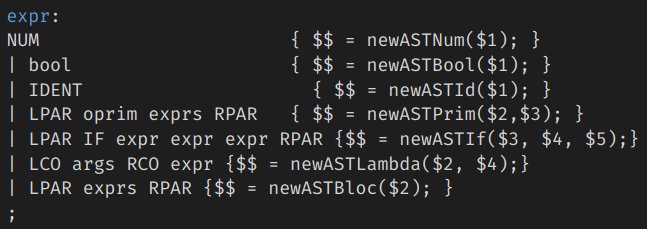
\includegraphics[width=0.5\textwidth]{grammar_expr.png}
			%\caption{fig1}
		\end{minipage}%
	}%
\end{figure}

\item AST. C'est une arbre d'analyse syntaxique. Dès qu'on a écrit la grammaire des expressions, l'interprèteur connaît la phrase, mais il ne fait rien. S'il veut la traiter, il a besoin de AST. Donc j'ai définit le noeud de AST \textbf{Expr} dans \textbf{ast.h} et réaliser les fonctions de constructeurs \textbf{newASTNum}, \textbf{newASTId}, \textbf{newASTBool}, \textbf{newASTPrim}, \textbf{newASTIf}, \textbf{newASTLambda}, \textbf{newASTBloc} et \textbf{appendExprs} dans \textbf{ast.c}. Puis appeler ces constructeurs dans \textbf{parser.y} dès qu'on a lu une phrase d'expression.\\

\item Prolog. Après construit AST, l'interprèteur peut le parcourir. Pour cet étape, on veut juste afficher AST d'expression en sortie standard. Donc il faut juste écrire la fonctions d'affichage pour chaque noeud de AST dans \textbf{prologTerm.c}.
\end{enumerate}

\clearpage
\subsubsection{Type et Arguments}
\textbf{Type} et \textbf{Arguments} est aussi bas niveau, donc je les réalise just après \textbf{Expr}.
\begin{enumerate}
	\item  Grammair. On ajoute la grammair pour comment exprimer un type dans le langage APS0. Dans notre langage, le type peut exprimé récursivement. Donc j'ai écrit la grammair comme l'image.
	\item AST. Ajouter les structures  \textbf{Type}, \textbf{Types}, \textbf{Arg} et \textbf{Args} dans \textbf{ast.h}, ainsi que les constructeur \textbf{newASTType} et \textbf{newASTArg} ainsi que \textbf{appendTypes} et \textbf{appendArgs} dans \textbf{ast.c}
	\item Prolog. Ajoute les fonctions d'affichage \textbf{printType}, \textbf{printTypes}, \textbf{printArg} et \textbf{printArgs} dans \textbf{prologTerm.c}
\end{enumerate}

\subsubsection{Statement}
Il n'y a qu'une seule instruction \textbf{ECHO Expr} dans APS0.
\begin{enumerate}
	\item  Grammair.  On ajoute la grammair de \textbf{ECHO} dans \textbf{paser.y}.
	\item AST. Ajouter les structures de \textbf{Stat} dans \textbf{ast.h}, ainsi que le constructeur dans \textbf{ast.c}
	\item Prolog. Ajoute la fonction d'affichage \textbf{printStat} dans \textbf{prologTerm.c}
\end{enumerate}

\subsubsection{Déclaration}
Il y a 3 types des déclarations dans APS0. On peut déclararer le constant, la fermeture et la fermeture récursive.
\begin{enumerate}
	\item  Grammair. On ajoute la grammair pour comment exprimer une déclaration. Dans notre langage, une déclaration commencée par son type, \textbf{CONST}, \textbf{FUN} ou \textbf{FUNREC}. 
	\item AST. Ajouter la structure de \textbf{Dec} dans \textbf{ast.h}, ainsi que son constructeur \textbf{newASTDec} dans \textbf{ast.c}
	\item Prolog. Ajoute la fonction d'affichage \textbf{printDec} dans \textbf{prologTerm.c}
\end{enumerate}

\subsubsection{Commande}
La commande est composée par la déclaration ou l'instruction, donc je code \textbf{Cmd} après réalise \textbf{Dec} et \textbf{Stat}.
\begin{enumerate}
	\item  Grammair. C'est plus simple que les grammaires précédentes, comme il n'y a plus de détail à décrire, une commande soit une déclaration soit une instruction.
	\item AST. Ajouter la structure de \textbf{Cmd} et \textbf{Cmds} dans \textbf{ast.h}, ainsi que son constructeur \textbf{newASTCmd} et \textbf{appendCmds} dans \textbf{ast.c}
	\item Prolog. Ajoute la fonction d'affichage \textbf{printCmd} et \textbf{printCmds} dans \textbf{prologTerm.c}
\end{enumerate}

\subsubsection{Programme}
Un programme de APS0 est une suite de commande.
\begin{enumerate}
	\item  Grammair. Un programme est une suite de commande dans une pair de crochet.
	\item AST. Ajouter la structure de \textbf{Proc} dans \textbf{ast.h}, ainsi que son constructeur \textbf{newASTProg} dans \textbf{ast.c}
	\item Prolog. Ajoute la fonction d'affichage \text{printProg} dans \textbf{prologTerm.c}
\end{enumerate}

\subsection{Etape3. Typage}
\subsubsection{Expression}
l'expression est la base du langage, donc je définit d'abord de type basique pour l'expression.
\begin{enumerate}
\item Le type des booléan, d'entier et des paramères de primitive ainsi que le type de résultat des primitives.
\item Le typage de \textbf{ASTIf}, il contient 3 expression: condition, résultat, alternance.
On garanti que le type de condition est booléan et les deux autres expression doit avoir le même type.
\item Le typage de l'application de fermeture.
\item Le typage de ABS
\end{enumerate}

\subsubsection{Déclaration}
\begin{enumerate}
	\item Déclaration de const est exprimé par const(id, type, expr). On doit garantir que le type de expression est aussi le type de identifiant dans l'environement G.
	\item Le typage de function et function récursive.
\end{enumerate}

\subsubsection{Statement}
le type de l'instruction est void. APS0 peut seulement afficher les entiers, donc on a juste besoin de garantir le type d'expression de \textbf{echo} est int. 

\subsubsection{Commande}
le type de la commande est void. la suite de commandes peut commencer par une déclaration ou une instruction.

\subsubsection{Program}
le type de program est aussi void.

\subsection{Etape4. Analyse sémantique}
\subsubsection{Définition de Value}
\textbf{Value} est la structure des données basique de APS0, elle soit un entier \textbf{inN}, soit une fermeture \textbf{inF}, soit une fermeture récursive \textbf{inFr}. Après l'exécution de l'expression, un résultat de \textbf{Value} est produit.

\subsubsection{Implémante structure de l'environement}
Je définit d'abord un struct \textbf{Env } dans \textbf{eval.h}. Il permet de conserver l'association entre les identifications et les valeur.

\subsubsection{Expr}
La fonction \textbf{evalExpr} est définit dans \textbf{eval.c}, cette fonction permet d'interprèter une expression et de rendre un résultat. Dans APS0, il y a 7 genres de l'expression.
\begin{enumerate}
\item Entier. C'est le type basique, juste rendre \textbf{inN}.
\item Identifiant. Il faut chercher la valeur qui correspond à cet identifiant dans l'environement et rendre cette valeur.
\item Booléan. Rendre inN(0) pour false et inN(1) pour true.
\item Primitives. Calculer le résultat en fonction de l'opération arithmétique.
\item If. Interprèter d'abord l'expression de condition. Si le résultat est positive, on interprète deuxième expression, sinon interprète la troisième.
\item Lambda. Rendre une \textbf{inF}.
\item AppFun. C'est la suite des expressions. Comme la règle du typage, on est sûr que la première expression est le nom de fermature, et les restes sont les valeurs des arguments.
On doit interprèter les restes d'expressions afin d'obtenir ces valeurs et ajouter à l'environement de la fermeture. A la fin on interprète la corps de fermeture avec son environement.

\end{enumerate}



 







\end{document}